\exer{Distance à partir d'une case du cavalier sur un échiquier}

Un cavalier se déplace, lorsque c'est possible, de 2 cases dans une direction verticale ou horizontale, et de 1 case dans l'autre direction (le trajet dessine une figure en L).


\begin{figure}[h]
	\begin{center}
		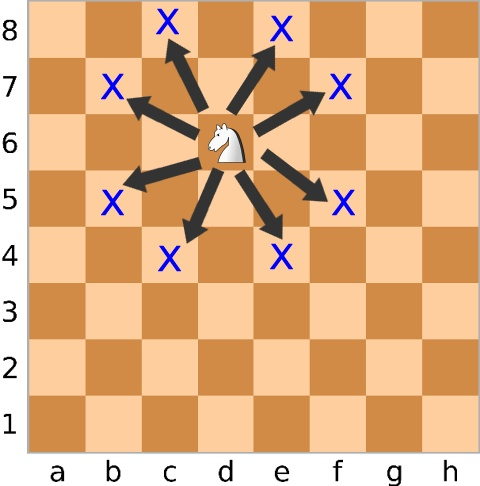
\includegraphics[width=0.3\linewidth]{deplacement-cavalier.jpg}
	\end{center}
	\caption{Illustration du mouvement d'un cavalier sur un échiquier}
\end{figure}


Les cases de l'échiquier sont représentées par des tuples~: le couple \texttt{(i, j)} désigne la case d'abscisse \texttt{i} et d'ordonnée \texttt{j}. Un échiquier possède 8 colonnes et 8 lignes, donc \texttt{i} et \texttt{j} seront compris entre \texttt{0} et \texttt{7}.

%Un fichier \texttt{cavalier\_etudiant.py} est dans votre espace de classe partagé.

%\begin{figure}[h]
%	\begin{center}
%		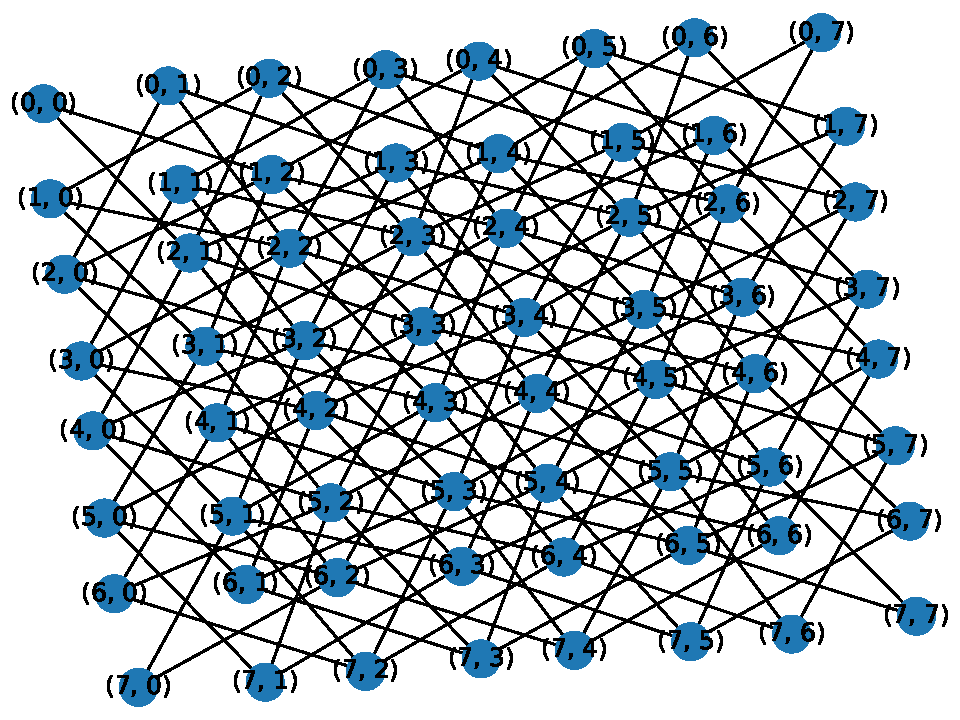
\includegraphics[width=0.7\linewidth]{Graphe_initial}
%	\end{center}
%	\caption{Représentation graphique du graphe \texttt{Gcav}}
%\end{figure}

\question{\'Ecrire une fonction \texttt{estDansEch(i:int, j:int)-> bool :} qui renvoie \texttt{True} si \texttt{(i, j)} correspond à une case valide de l'échiquier et \texttt{False} sinon.}

\question{\'Ecrire une fonction \texttt{mvtsPossibles(i:int, j:int)} qui renvoie la liste des cases (sous forme de tuple) où le cavalier peut se déplacer à partir de la case \texttt{(i, j)} à l'ordre après.}


\question{Vérifier que~:
\begin{itemize}
	\item \texttt{mvtsPossibles(0, 0)} renvoie \texttt{[(1, 2), (2, 1)]},
	\item \texttt{mvtsPossibles(3, 5)} renvoie bien \texttt{[(1, 4), (1, 6), (2, 3), (2, 7), (4, 3), (4, 7), (5, 4), (5, 6)]},
	\item \texttt{mvtsPossibles(7, 7)} renvoie bien \texttt{[(5, 6), (6, 5)]}.
\end{itemize}
Tous ces résultats sont à l'ordre près.}

\question{\'Ecrire une fonction  \texttt{make\_graphe} renvoyant un graphe ayant pour sommets les différentes cases de l'échiquier et pour arêtes le mouvement possible du cavalier. Le graphe sera un dictionnaire donc les clefs seront des tuples correspondant aux cases de l'échiquier. Les valeurs associées seront des listes de tuples correspondant aux positions accessibles.}

\question{\'Ecrire une fonction \texttt{largeur\_dist(G, dep)} qui prend en entrée un graphe codé par un dictionnaire d'adjacence \texttt{G} et un sommet de départ \texttt{dep} et renvoie un dictionnaire de distances à partir du sommet \texttt{dep}. Pour ce faire, vous vous inspirerez du parcours en largeur fourni. Si un sommet n'est pas atteignable depuis le depuis \texttt{dep}, la valeur associée doit être de \texttt{-1}.}

%Quelques fonctions de \texttt{matplotlib}~: 
%\begin{itemize}
%	\item \texttt{plt.text(x, y, s)} permet de placer la chaine de caractère \texttt{s} aux coordonnées \texttt{(x, y)}~;
%	\item  \texttt{plt.axis("off")} permet de rendre les axes invisibles~;
%	\item \texttt{plt.xlim([xmin, xmax])} permet de régler l'affichage des abscisses~; 
%	\item \texttt{plt.ylim([ymin, ymax])} permet de régler les ordonnées. 
%\end{itemize}

%\UPSTIquestion Représenter dans une liste de liste \texttt{M} les différentes distances lorsque le départ est à \texttt{(0, 0)}, puis lorsque le départ est à \texttt{(4, 3)}. \texttt{M[i][j]} doit correspondre à la distance du sommet initial choisi jusqu'à la case \texttt{(i,j)}. 

\question{Vérifier que vous obtenez le même résultat que sur la figure \ref{fig:verif} en affichant les différentes valeurs de distance depuis \texttt{dep = (0, 0)} et \texttt{dep = (4, 3)}. La fonction \texttt{print} peut ne pas revenir à la ligne si on précise un argument optionnel \texttt{end} différent de \texttt{\textbackslash n}. Suivant vos implémentations, la table des distances peut être << orientée >> différemment. }

\begin{figure}[h]
	\begin{center}
		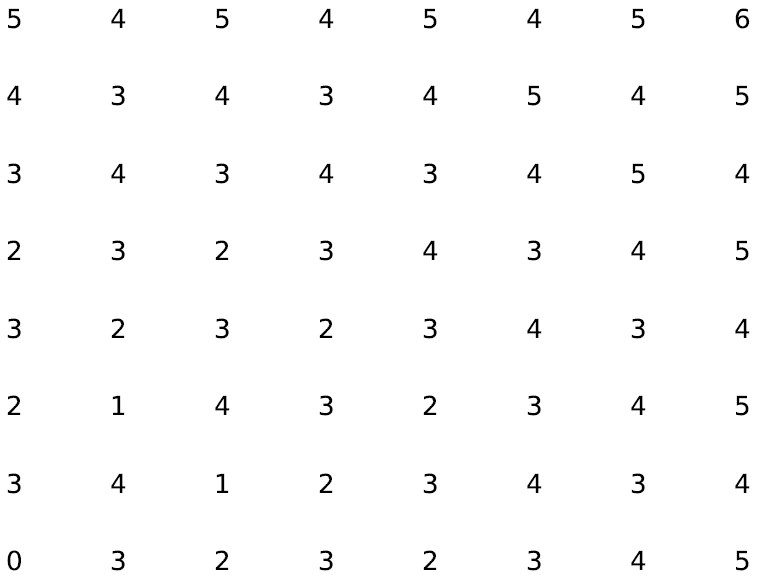
\includegraphics[width=0.44\linewidth]{distance_0_0.jpg}
		\hfill
		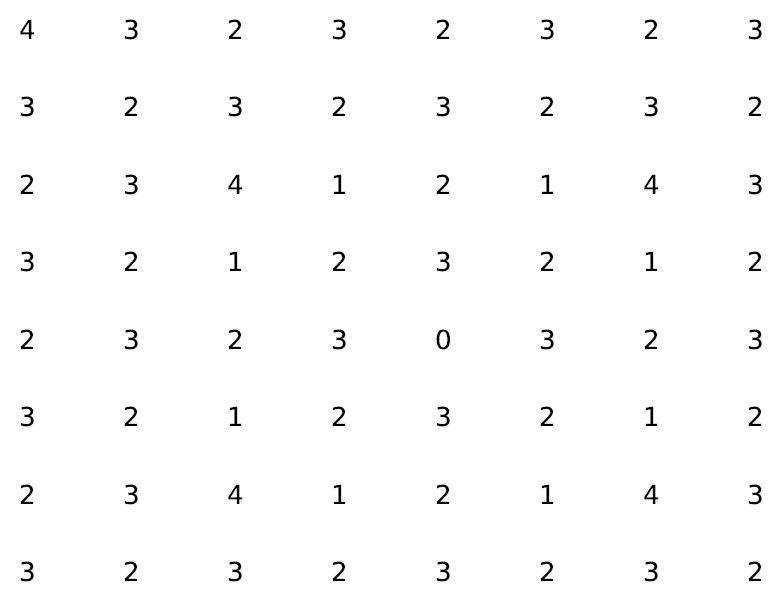
\includegraphics[width=0.45\linewidth]{distance_4_3.jpg}
	\end{center}
	\caption{Distances depuis \texttt{(0, 0)} et \texttt{(4, 3)}}
	\label{fig:verif}
\end{figure}

\question{Pourquoi le parcours en profondeur n'est pas adapté à la résolution de ce problème~?}

%\UPSTIquestion Représenter la moyenne des distances de toutes les cases pour chaque départ~: on utilisera un arrondi à 2 chiffres après la virgule (fonction \texttt{round}). 

%
%\begin{figure}[h]
%	\begin{center}
%		\includegraphics[width=0.7\linewidth]{MouvementsCavalier/distance_moy}
%	\end{center}
%	\caption{Moyenne des distances des autres cases à partir d'une case donnée}
%	\label{fig:verif}
%\end{figure}








